\documentclass[11pt,a4paper]{article}
\usepackage[T1]{fontenc}
\usepackage[utf8]{inputenc}
\usepackage{lmodern,microtype,amsmath,amssymb,booktabs,longtable,array,graphicx}
\usepackage[margin=23mm]{geometry}
\usepackage{xcolor,tikz,fancyhdr,enumitem}
\usetikzlibrary{arrows.meta,positioning}
\definecolor{navy}{HTML}{0F1E2E}
\definecolor{teal}{HTML}{0D8080}
\definecolor{ice}{HTML}{EEF5F5}
\usepackage[colorlinks=true,linkcolor=teal,urlcolor=teal,citecolor=teal]{hyperref}
\hypersetup{pdftitle={Mini-IPHOREOS: Mathematical Model and Engineering Realisation},pdfauthor={Mini-IPHOREOS project}}
\pagestyle{fancy}\fancyhf{}\fancyhead[L]{\small\textcolor{teal}{MINI-IPHOREOS / MATHEMATICAL COMPANION}}
\fancyfoot[L]{\small From belief to physical movement}\fancyfoot[R]{\thepage}
\setlength{\headheight}{15pt}
\setlength{\parindent}{0pt}\setlength{\parskip}{6pt}
\setlist{itemsep=3pt,topsep=4pt}
\newcommand{\code}[1]{\texttt{\detokenize{#1}}}
\setlength{\emergencystretch}{2em}
\newcommand{\tuto}[2]{\par\textcolor{teal}{\textbf{Do this in the tutorial:}} Chapter #1, #2. See the \href{Tutorial_A_to_Z.html\#t#1}{browser chapter} or \href{Tutorial_A_to_Z.pdf}{PDF tutorial}.\par}
\newcommand{\N}{\mathcal N}
\begin{document}
\begin{titlepage}
\textcolor{teal}{\large IPHOREOS / CONCEPT--EVENT--CONTEXT--POLICY}\par
\vspace{14mm}
{\Huge\bfseries\color{navy} The mathematical model\\[3mm] of a small working robot\par}
\vspace{5mm}
{\Large Mini-IPHOREOS: belief estimation, short-pulse control, verification and engineering realisation\par}
\vspace{7mm}
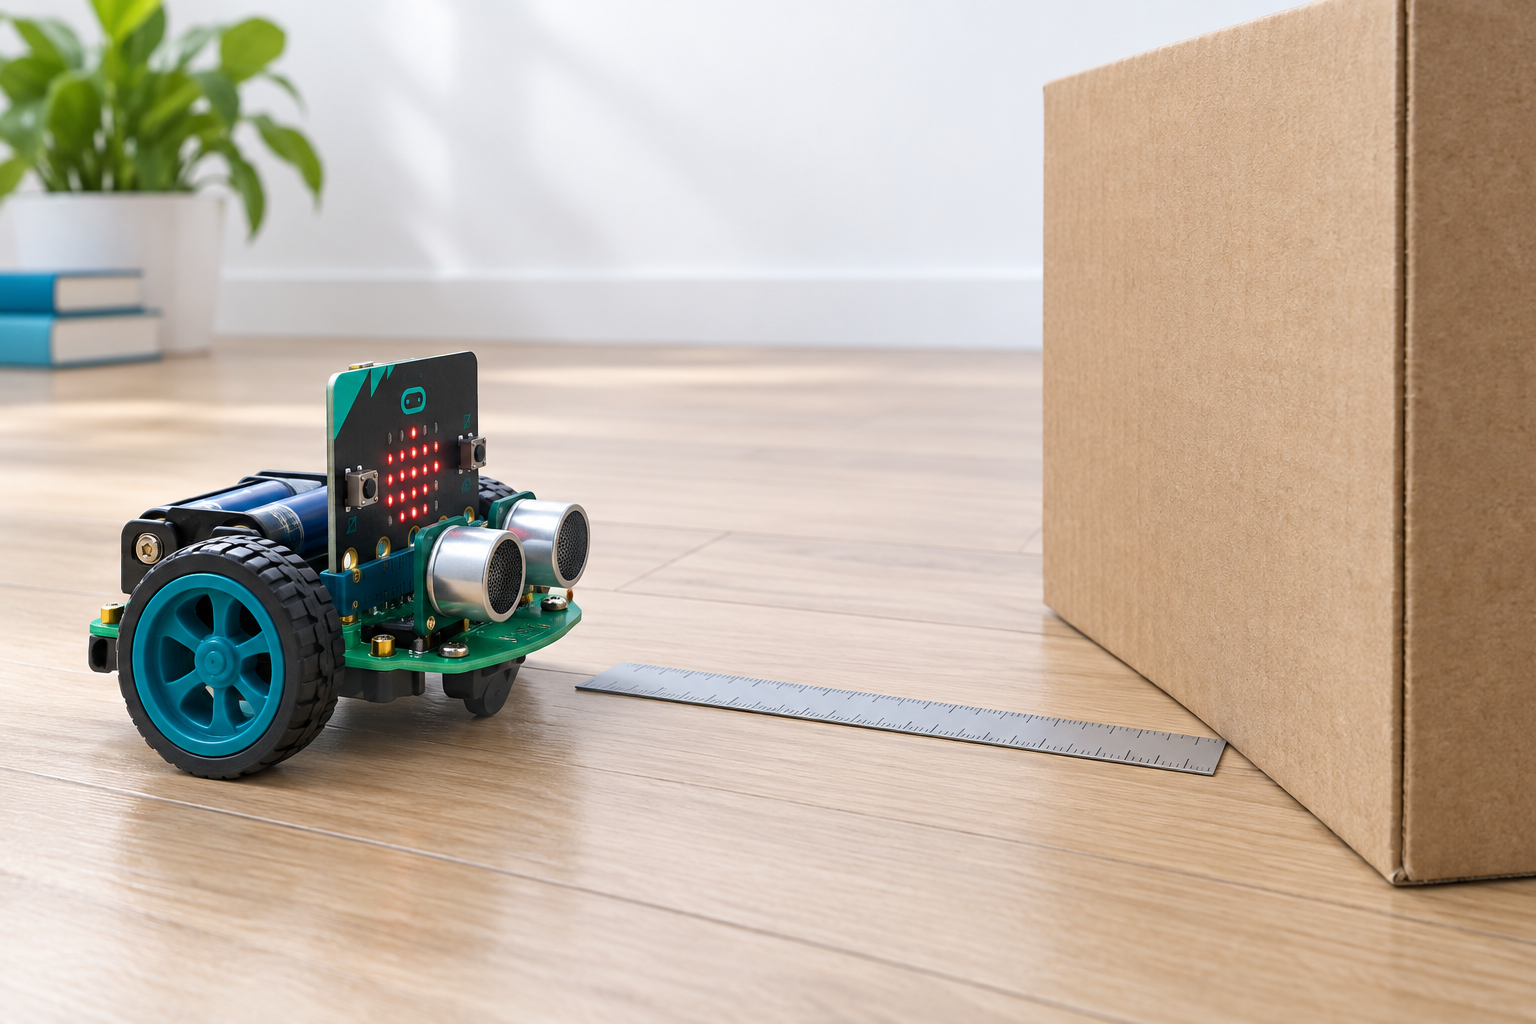
\includegraphics[width=\linewidth,height=70mm,keepaspectratio]{assets/robot_concept.png}
\par{\small AI-generated concept illustration; not a photograph or an assembly drawing.\par}
\vspace{7mm}
\colorbox{ice}{\parbox{.95\linewidth}{\textbf{One observable task.} Approach a cardboard wall and verify that the ultrasonic sensor face is within 21--29 cm of it, with a nominal target of 25 cm.}}\par
\vspace{5mm}
This companion derives the equations, documents the implemented decisions, explains calibration, and connects every stage to the practical build tutorial. It distinguishes implemented behaviour from possible research extensions.

\textbf{Start with:} \href{Tutorial_A_to_Z.pdf}{the illustrated A--Z tutorial} or \href{index.html}{the project homepage}. Keep this PDF beside those files so relative links resolve. Some PDF readers require permission to open local links; the printed chapter numbers remain usable.

\vfill
Prepared for Florent Ouabo Kamkumo\\
10 September 2026 / Implementation companion v1.0\\
\textbf{Status:} computer-tested software; physical calibration and validation pending.
\end{titlepage}
\tableofcontents
\newpage
\section{The task, the mathematical question and the answer}
The mathematical question is: \emph{given an uncertain distance measurement and an imperfect movement model, should the robot move a little, measure again, or stop?} The answer implemented here is a scalar Bayesian estimator inside a bounded state machine.

The physical objective uses true distance $d$, not the sensor output:
\begin{equation}
 d_\star=25\ \mathrm{cm},\qquad \varepsilon=4\ \mathrm{cm},\qquad
 \mathcal T=[d_\star-\varepsilon,d_\star+\varepsilon]=[21,29]\ \mathrm{cm}.
\end{equation}
Success means the controller reports \code{DONE} and an independent measurement confirms $d\in\mathcal T$. A happy-face display alone establishes only the controller's conclusion.

We deliberately reduce the mechanics to one dimension. The robot begins approximately facing a broad, stationary cardboard wall, moves forward only, and measures while stopped. There is no steering controller, encoder feedback, arm, object recognition or autonomous reverse recovery. Wheel mismatch, angled echoes, slipping and moving targets can invalidate this reduction.

\begin{center}
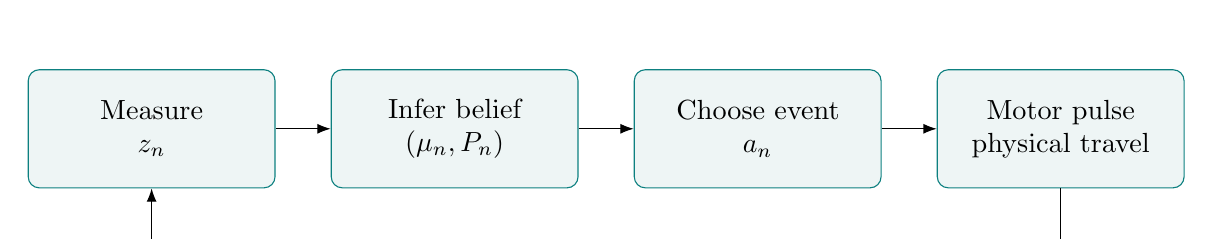
\begin{tikzpicture}[>=Latex,box/.style={draw=teal,fill=ice,rounded corners,text width=29mm,align=center,minimum height=15mm},node distance=7mm]
\node[box](s){Measure\\$z_n$};\node[box,right=of s](b){Infer belief\\$(\mu_n,P_n)$};
\node[box,right=of b](a){Choose event\\$a_n$};\node[box,right=of a](m){Motor pulse\\physical travel};
\draw[->](s)--(b);\draw[->](b)--(a);\draw[->](a)--(m);
\draw[->](m.south)--++(0,-8mm)-|(s.south);
\end{tikzpicture}
\end{center}
\textbf{The engineer's deliverable} is a measured mapping from command to travel and a trustworthy distance observation. \textbf{The mathematician's deliverable} is an estimator, decision rule, assumptions and experiment definitions that use that mapping. The software--hardware interface is therefore explicit and testable.
\tuto{01}{Understand the finished project; chapter 07 explains the physical interface}

\section{Variables, units and the complete internal state}
Use centimetres and seconds throughout this implementation. When integrating with an SI-based robotics stack, use $d_{\rm m}=d_{\rm cm}/100$ and $P_{\rm m^2}=P_{\rm cm^2}/10^4$.
\begin{longtable}{p{.17\linewidth}p{.55\linewidth}p{.18\linewidth}}
\toprule Symbol & Meaning & Unit\\\midrule\endhead
$n$ & Observation/decision index; increments even when stopped & dimensionless\\
$d_n$ & True sensor-face-to-wall distance, hidden from controller & cm\\
$z_n$ & Raw ultrasound-derived reading before bias correction & cm\\
$b,\hat b$ & Actual additive sensor bias and calibrated estimate & cm\\
$y_n=z_n-\hat b$ & Corrected reading & cm\\
$\mu_n,P_n$ & Estimated mean and variance after accepted observation & cm, cm$^2$\\
$\mu_n^-,P_n^-$ & Prior mean and variance before that observation & cm, cm$^2$\\
$R,Q$ & Assumed measurement variance and variance added per pulse & cm$^2$\\
$P_{\min}$ & Numerical uncertainty floor & cm$^2$\\
$\hat v,\tau,\hat c$ & Calibrated speed, pulse duration and coast distance & cm/s, s, cm\\
$m$ & Additional heuristic movement margin & cm\\
$\kappa$ & Context-dependent uncertainty multiplier & dimensionless\\
$a_n$ & SAMPLE, MOVE, DONE or ABORT & event\\
\bottomrule
\end{longtable}
The Gaussian pair is not the entire controller state. The software additionally stores observation counters, move count, verification count, a stop latch for the baselines, a progress anchor, terminal status and the first observation time. Denote this augmented state by
\[
 S_n=(\mu_n,P_n,N_s,N_m,N_v,N_i,N_r,L,A,T,t_0).
\]
Here $N_s$ counts observations since the last move, $N_i$ invalid observations and $N_r$ rejected innovations; $L$ is the stop latch and $A$ the progress anchor. Decisions depend on these variables as well as the belief. Thus the controller is Markovian in $S_n$ given the next reading and time, rather than in distance belief alone.

\section{From ultrasound time to a distance observation}
An ultrasonic echo measures a round trip. If sound speed is $c_{\rm sound}$ and the measured duration is $t_e$, the ideal distance is
\begin{equation}
 d=\frac{c_{\rm sound}t_e}{2}.
\end{equation}
The adapter uses a nominal conversion
\begin{equation}
 z_n\ [\mathrm{cm}]=\frac{t_e\ [\mu\mathrm{s}]}{58}.
\end{equation}
For example, $1450\ \mu$s gives $25$ cm. This factor is a starting calibration convention, not a temperature compensation model. Trigger P13 is held low for 5 microseconds and high for 10 microseconds; P14 is timed with \code{time_pulse_us(pin14,1,12000)}. The MicroPython API reports negative values for timeout conditions \cite{microbit}. The 12,000-microsecond timeout applies to the API's waiting/timing phases, not a certified upper bound on the entire sensing routine.

The adapter returns no reading for a nonpositive duration or a converted value outside 2--150 cm. The controller then applies its stricter 12--150 cm raw acceptance interval. Consequently, a physical distance below the adapter's 2 cm limit can appear as a missing observation, rather than as an immediate numeric clearance violation. This is one reason not to interpret these guards as independent obstacle protection.

The working observation model for accepted readings is
\begin{equation}\label{eq:obs}
 z_n=d_n+b+\nu_n,\qquad y_n=d_n+(b-\hat b)+\nu_n,
 \qquad \nu_n\overset{\rm model}{\sim}\N(0,R).
\end{equation}
The estimator assumes the residual bias $b-\hat b$ is negligible and noise is independent of prior state error. Dropouts and large outliers are handled by guards outside this Gaussian model. An angled wall or distance-dependent bias is not repaired by averaging more measurements.
\tuto{09}{First experiment: measure without moving}

\section{The movement model and its physical meaning}
Let $u_n=1$ for an executed forward pulse and $u_n=0$ for stationary sampling. A local physical model is
\begin{equation}\label{eq:dynamics}
 d_{n+1}=d_n-u_n(v\tau_n+c)+w_n.
\end{equation}
Here $v$ is effective forward speed under the selected PWM, $c$ is travel after motor-off, and $w_n$ represents movement error. This simple relation is appropriate only over the calibrated operating range. It is not a full DC motor dynamics model.

For a successfully completed pulse, the implemented prediction is
\begin{align}
 \mu_{n+1}^-&=\mu_n-\hat v\tau_{\rm actual}-\hat c,\label{eq:predictmean}\\
 P_{n+1}^-&=P_n+Q.\label{eq:predictvar}
\end{align}
With defaults, $\hat v=8$, $\tau=0.12$ and $\hat c=0.15$, expected travel is $1.11$ cm. $Q=0.64$ cm$^2$ is added once per pulse, regardless of the measured pulse duration. For SAMPLE, the state is predicted unchanged: there is no added stationary process noise. This assumes the robot and wall do not drift while waiting.

The decision rule predicts travel using configured $\tau=0.12$ s, whereas \code{record_move} uses measured elapsed adapter time. That elapsed time includes some driver and stop-call overhead; it is not encoder-measured powered travel. The adapter limits requested pulses to 250 ms and PWM values to 80, checks button B during the pulse, and calls motor-off in a \code{finally} block. The controller accepts a reported duration up to 300 ms. These different limits accommodate overhead; they do not establish an exact bound on real travel.

After a pulse, the main program waits 200 ms before measuring. The settling time must exceed observed coast time. Failure to settle invalidates the stopped-measurement model. On cancellation or exception, the trial exits instead of resuming estimation from an unmodelled partial pulse.
\tuto{10}{First movement: one supported-wheel pulse; then chapter 11 for floor calibration}

\section{Deriving the scalar Bayesian update}
Before an accepted reading, represent distance uncertainty by the working belief
\[
 q_n^-(d)=\N(d;\mu_n^-,P_n^-).
\]
Under the bias-corrected likelihood $p(y_n\mid d)=\N(y_n;d,R)$, Bayes' rule gives
\begin{equation}
 q_n(d)\propto \exp\left[-\frac12\left\{\frac{(d-\mu_n^-)^2}{P_n^-}+\frac{(y_n-d)^2}{R}\right\}\right].
\end{equation}
Collecting the quadratic and linear terms in $d$ yields
\begin{equation}
 \widetilde P_n=\left(\frac1{P_n^-}+\frac1R\right)^{-1},\qquad
 \mu_n=\widetilde P_n\left(\frac{\mu_n^-}{P_n^-}+\frac{y_n}{R}\right).
\end{equation}
Equivalently, with Kalman gain $K_n$,
\begin{align}
 K_n&=\frac{P_n^-}{P_n^-+R},\\
 \mu_n&=\mu_n^-+K_n(y_n-\mu_n^-),\label{eq:update}\\
 P_n&=\max\{P_{\min},(1-K_n)P_n^-\}.\label{eq:floor}
\end{align}
The scalar linear-Gaussian update is a special case of recursive linear filtering \cite{kalman}; the variance floor and rejection rules are project-specific engineering modifications. Once those modifications or biased/correlated observations apply, the stored Gaussian is an approximate belief, not an exact posterior with guaranteed coverage.

\textbf{Initialisation.} There is no encoded start-position prior. The first accepted reading sets $\mu_0=y_0$ and $P_0=R$. It is not processed a second time as an independent measurement.

\textbf{Stationary sampling.} Without the floor, $j$ further independent readings give $P_j=(1/P_0+j/R)^{-1}$. With $P_0=R$, this is $R/(j+1)$. The floor $P_{\min}=0.36$ prevents a stored standard deviation below $0.6$ cm. The mean continues updating after the floor is reached: the gain remains positive. This is not bias learning.

\textbf{Interpretation.} A large $P_n^-$ makes a new measurement more influential; a large $R$ makes it less influential. $R$ and $P$ are variances, not standard deviations. Entering a 2 cm standard deviation as $R=2$ instead of $R=4$ changes the controller.
\tuto{13}{Understand the model you are running}

\section{Observation guards and their exact scope}
Before the update, \code{Controller.observe} applies these tests in order:
\begin{enumerate}
\item If a terminal status already exists, return it unchanged. Otherwise initialise $t_0$ on the first call and abort if $t-t_0\geq60$ s.
\item Increment $N_s$. A missing, nonfinite or out-of-range raw value increments $N_i$ and clears verification. A finite raw value below 12 cm aborts immediately. Other invalid readings cause SAMPLE, or ABORT when $N_i\geq3$ or $N_s>16$.
\item Correct the bias. A corrected value below 12 cm aborts immediately. There is no second upper-range check after bias correction in the current implementation.
\item If a belief exists, reject the observation when
\begin{equation}
 |y_n-\mu_n^-|>\max\left\{8,\;4\sqrt{P_n^-+R}\right\}\ \mathrm{cm},
\end{equation}
where all numeric terms are evaluated in centimetres. Increment $N_r$, clear verification, and SAMPLE; ABORT at $N_r\geq3$ or $N_s>16$.
\item On an accepted reading, reset both $N_i$ and $N_r$ and perform the update.
\end{enumerate}
These failure counters reset on an \emph{accepted} observation. Alternating invalid and rejected readings need not be three identical consecutive errors to trigger one of their limits. Invalid and rejected branches do not update the belief. Because they use $N_s>16$ while the accepted branch later uses $N_s\geq16$, a run of mixed unusable observations can reach a seventeenth observation before that particular limit aborts.

The innovation gate protects against isolated implausible returns but can also reject a real abrupt change. It is a failure detector, not a method of tracking arbitrary moving obstacles.

\section{Verification: what DONE means mathematically}
For Mini, define the working interval
\begin{equation}
 I_n=[\mu_n-\kappa\sqrt{P_n},\;\mu_n+\kappa\sqrt{P_n}].
\end{equation}
The interval is contained in the target band exactly when
\begin{equation}\label{eq:verify}
 |\mu_n-d_\star|+\kappa\sqrt{P_n}\leq\varepsilon.
\end{equation}
To see this, require its lower endpoint to be at least $d_\star-\varepsilon$ and its upper endpoint at most $d_\star+\varepsilon$, then combine the two inequalities.

Normal context uses $\kappa=1.64$ and careful context $\kappa=2.33$. For a genuinely calibrated Gaussian these intervals contain approximately 89.9\% and 98.0\% probability respectively. The corresponding \emph{one-sided} tail probabilities are approximately 5.05\% and 0.99\%. Do not confuse a central interval probability with a one-sided tail probability.

If the Gaussian assumption holds, the exact target probability is
\begin{equation}
 p_{\mathcal T}=\Phi\left(\frac{29-\mu_n}{\sqrt{P_n}}\right)-
 \Phi\left(\frac{21-\mu_n}{\sqrt{P_n}}\right).
\end{equation}
Interval containment is a sufficient condition for $p_{\mathcal T}\geq2\Phi(\kappa)-1$ under that model, not a necessary condition. The firmware evaluates the simpler inequality, not $\Phi$.

Every successful verification test increments $N_v$. The first two return SAMPLE; the third returns DONE. An unsuccessful verification, rejected/invalid observation or completed movement clears $N_v$. Repeated posteriors share history, so three confirmations are not three independent safety certificates and their probabilities must not be multiplied.

At the variance floor, the maximum allowed mean error is $4-0.6\kappa$: 3.016 cm in normal mode and 2.602 cm in careful mode. Thus the target is a band, not a demand to reach exactly 25 cm.
\tuto{14}{Understand the four events; chapter 18 explains independent measurements}

\section{The implemented Mini movement decision}
Verification is attempted before movement. If it has not succeeded, the algorithm applies limits and constructs
\begin{equation}\label{eq:lower}
 \Delta=\hat v\tau+\hat c,\qquad
 L_n=\mu_n-\kappa\sqrt{P_n}-\Delta-m.
\end{equation}
For Mini, a move is permitted only when
\begin{equation}\label{eq:move}
 L_n\geq21\ \mathrm{cm}\quad\text{and}\quad\mu_n>25\ \mathrm{cm},
\end{equation}
provided preceding guards and limits have passed. Otherwise it requests SAMPLE. Here $m=0.5$ cm is an extra chosen margin. SAMPLE means motors off, wait 150 ms, and obtain another observation. It does not mean a motor micro-adjustment.

The distinction between prediction and uncertainty matters: equation~\eqref{eq:lower} uses $\sqrt{P_n}$, \emph{not} $\sqrt{P_n+Q}$. $Q$ is added only after movement in equation~\eqref{eq:predictvar}. The rule also lacks an explicit bound on residual bias, motor timing error or coast variation. It is therefore an uncertainty-aware heuristic, not an implemented chance-constrained safety proof.

\textbf{Possible future rule, not implemented.} Under a Gaussian next-state model, a one-step lower-tail condition would instead take the form
\begin{equation}\label{eq:future}
 \mu_n-\Delta-\kappa\sqrt{P_n+Q}-B-E\geq21,
\end{equation}
where $B$ and $E$ are validated bounds for residual bias and systematic travel error. Such a rule would require new calibration and policy tests; changing one square root alone would not certify a robot. The 21 cm threshold is the near edge of the target band, not the physical collision boundary at $d=0$.

\textbf{Bounded waiting.} On the accepted-observation path, if verification does not succeed and $N_s\geq16$, ABORT. If a baseline stop latch is active, SAMPLE next; otherwise abort at $N_m\geq80$ before considering movement. Verification comes first, so a final successful confirmation is allowed at a count boundary.

\textbf{Progress check.} An anchor is set at the first accepted mean. When $N_m$ is a nonzero multiple of eight \emph{and} $N_s=1$ on an accepted observation, require anchor minus current mean to be at least 1 cm; otherwise ABORT. Then reset the anchor. This is a sparse check. If the first observation after the eighth pulse is invalid, that block's check is skipped because later observations have $N_s>1$.

DONE and ABORT are absorbing states. The main program turns motors off and exits the active trial. There is no automatic reverse or restart; reposition and begin a new trial explicitly.

\section{Three policies and the role of context}
All three policies share the observation model, guards and limits; even the raw baseline maintains a belief for its innovation/progress guards. They differ in the decision rules below.
\begin{longtable}{p{.13\linewidth}p{.36\linewidth}p{.40\linewidth}}
\toprule Policy & Stop/verification & Movement when not verifying\\\midrule\endhead
Raw & Latch stop once $y\leq25$; then require $|y-25|\leq4$ for three accepted confirmations. & Forward pulses until latched or another guard/limit stops the trial.\\
Belief & Latch stop once $\mu\leq25.5$; then require $|\mu-25|+1.64\sqrt P\leq4$. & Forward pulses until latched or stopped; no Mini lower-bound test.\\
Mini & No stop latch; verify using equation~\eqref{eq:verify}. & Apply equations~\eqref{eq:lower}--\eqref{eq:move}.\\
\bottomrule
\end{longtable}
Context is selected before a trial; it is not estimated online. Only Mini's decision uses the selected $\kappa$. The belief baseline always uses 1.64, and raw ignores context. This explains duplicate baseline rows across contexts in the synthetic results.

In the main IPHOREOS vocabulary, the toy's \emph{concept} is distance-to-target with uncertainty, \emph{events} are the four actions, \emph{context} sets $\kappa$, and \emph{policy} maps augmented belief state to an event. It retains belief-dependent action and verification. It omits learned concepts, inferred contexts, task hierarchies, episodic memory and expected-free-energy optimisation.

One may interpret repeated sensing as information gathering: for the unmodified Gaussian update, its expected entropy reduction is $\frac12\log(1+P^-/R)$. The current program does not compute this quantity or optimise a weighted information/task objective. Calling it a full active-inference solver would overstate the implementation.
\tuto{15}{Add a reduced context philosophy; chapter 17 compares the three versions}

\section{Worked calculations you can reproduce}
\subsection{A prediction--measurement cycle}
Suppose an accepted reading initialises $(\mu,P)=(50,4)$. Mini requests MOVE, since $50-1.64(2)-1.11-0.5=45.11\geq21$. After an actual 0.12 s pulse,
\[
 \mu^-=48.89,\qquad P^-=4.64.
\]
For a new corrected reading of 49 cm, $K=4.64/8.64=0.537037$, hence
\[
 \mu=48.949074\ \mathrm{cm},\qquad P=2.148148\ \mathrm{cm}^2.
\]
This is a constructed arithmetic example, not a real robot measurement.

\subsection{Same measurement, different context}
The first reading is 26 cm, so $\mu=26$, $\sqrt P=2$. Normal verification fails because $1+1.64(2)=4.28>4$. But the predicted lower value is $26-3.28-1.11-0.5=21.11$, so normal requests MOVE. Careful verification also fails and its lower value is $26-4.66-1.11-0.5=19.73$, so careful requests SAMPLE. The context changes an action through a specific inequality, not an unexplained label.

\subsection{Three confirmations}
With three consecutive 25 cm readings in normal mode, the posterior pairs are $(25,4)$, $(25,2)$ and $(25,4/3)$. Each interval fits the band. The actions are SAMPLE, SAMPLE, DONE. With no action between them, the default model adds no process noise. Careful context fails the first test ($2.33\cdot2>4$), then requires three successful confirmations starting at the second observation.

\subsection{Confidence can be wrong}
If true distance is 20 cm and residual bias is +5 cm, repeated readings near 25 cm can lead to a narrow belief and DONE outside the true band. No variance floor or repetition count identifies an unmodelled constant bias by itself. The next section explains why an independent ruler reference is essential.

The supplied \code{tools/check_math_model.py} evaluates these examples against the actual shared controller and records numeric results in \code{results/math_model_checks.json}.

\section{Calibration as parameter estimation}
\subsection{Sensor bias and measurement variance}
At measured ruler distances $d_i^{\rm ref}$, collect raw observations $z_i$ and form residuals $e_i=z_i-d_i^{\rm ref}$. The current calibration tool computes
\begin{equation}
 \hat b=\bar e=\frac1N\sum_i e_i,\qquad
 \hat R=\max\left\{0.1,\frac1{N-1}\sum_i(e_i-\bar e)^2\right\}.
\end{equation}
The tool requires at least ten rows; the tutorial recommends 20 readings at each of 20, 30, 40 and 60 cm, with a held-out check at 45 cm. Its CSV unit is cm. Pooling is justified only if residual bias/variance are reasonably stable over distance. Plot residuals by distance and order; a trend calls for a better calibration model, and serial correlation calls for more conservative uncertainty treatment.

Ruler alignment and reference uncertainty contribute to these residuals. If independent reference error has known variance $R_{\rm ref}$, the residual variance contains both sensor and reference contributions; the provided tool does not separate them. The standard error $\sqrt{\hat R/N}$ describes bias estimation only under independent, representative samples, and the firmware does not automatically add that bias uncertainty to $P$.

\subsection{Travel per pulse}
For repeated trials under fixed PWM/floor/battery conditions, record powered time $\tau_i$, powered travel $\ell_i$, and coast $c_i$. The tool reports
\begin{equation}
 \hat v=\frac1J\sum_i\frac{\ell_i}{\tau_i},\qquad
 \hat c=\frac1J\sum_i c_i,\qquad
 \hat Q=\operatorname{sampleVar}(\ell_i+c_i).
\end{equation}
It also reports maximum observed coast. At least five trials are required; more repetitions across expected battery conditions give a more useful estimate. The pooled travel variance is meaningful for a fixed pulse duration. If duration varies, a preferable future estimate is residual variance about a fitted travel model, rather than variance of mixed-duration distances. That regression is not implemented by this tool.

If powered travel and coast cannot be separated reliably, use total travel divided by the fixed pulse duration as effective speed and set coast to zero, as described in the tutorial. Do not also add coast, which would double-count it. This effective model is local to the calibrated pulse duration.

\subsection{Identifiability and model checking}
From stationary data $z=d+b+\nu$ alone, the pair $(d,b)$ is unidentifiable: replacing it by $(d+\delta,b-\delta)$ leaves the likelihood unchanged. Repeated samples improve precision about $d+b$, not identification of $d$. Likewise, one fixed-duration travel experiment identifies $v\tau+c$, not $v$ and $c$ separately. Independent distance references and either coast observations or varied-duration experiments resolve those ambiguities.

Choose $P_{\min}$, $m$ and operating limits conservatively from held-out behaviour; the tool does not infer them. Its JSON includes metadata as well as parameters. Transfer only relevant parameter fields to \code{CALIBRATION}, rather than passing the entire JSON to \code{Controller}, which rejects unknown keys. Neither the tool nor this document enables motors automatically.
\tuto{11}{Calibrate the physical model; chapter 12 enters and checks the estimates}

\section{From the mathematical action to motor power}
For a differential-drive robot with wheel radius $r$, wheel separation $B_w$ and angular speeds $\omega_L,\omega_R$, ideal no-slip kinematics give
\begin{equation}
 v=\frac r2(\omega_L+\omega_R),\qquad
 \dot\theta=\frac r{B_w}(\omega_R-\omega_L).
\end{equation}
The one-dimensional approximation assumes heading error remains small and $\dot d\approx-v$. Matching numeric PWM values does not guarantee equal wheel speeds. Use supported-wheel tests and measured straight travel to assess the assumption; the current code has no feedback correction for heading.

\textbf{Command chain.} The event MOVE reaches \code{Robot.pulse(left,right,milliseconds)}. It calls the vendor driver for left and right forward motor operation, waits briefly while checking B, and switches both channels off. The on-board motor electronics supply energy from the batteries. The mathematical variable $\hat v$ is a calibrated consequence of that chain; sending the number 8 to a motor API would not mean 8 cm/s.

PWM 45 is a provisional vendor-scale command (0--255), while this project's training cap is 80. It is not directly a voltage measurement or a guaranteed duty-cycle/speed relation. Load, supply voltage, friction and controller electronics intervene. Use the kit's integrated driver rather than supplying motors from micro:bit signal pins.

\begin{longtable}{p{.25\linewidth}p{.35\linewidth}p{.30\linewidth}}
\toprule Mathematical operation & Software location & Engineering evidence\\\midrule\endhead
$z=t_e/58$ & \code{firmware/hardware.py}, distance & Known-distance readings\\
$\mu,P$ update and guards & \code{belief_controller.py} in \code{firmware/}, observe & Desktop examples and ruler errors\\
Event to pulse & \code{firmware/main.py}, MOVE branch & Supported wheels, measured duration\\
$\mu^-\!,P^-$ prediction & Controller, record\_move & Measured travel/coast\\
Calibration values & \code{firmware/config.py} & Recorded CSVs and held-out checks\\
Independent truth in experiments & \code{simulate.py}, or physical ruler & Never reuse estimate as ground truth\\
\bottomrule
\end{longtable}
Logs are emitted before the chosen action is executed. A MOVE row therefore records the pre-movement posterior, not the new predicted position. Hardware time is emitted in milliseconds and simulation time in seconds; convert before comparing. Software printing does not by itself create a stored onboard experiment file.

PicoGK is a geometry kernel for computational engineering \cite{picogk}. A later design could translate bracket dimensions, sensor clearances and enclosure constraints into geometry. Our proposed use is an optional mechanical design extension; it is not part of this kit's runtime control path. Changing geometry would require revisiting sensor reference position and motion calibration.
\tuto{07}{See exactly how software moves hardware; chapter 08 covers programming}

\section{Default parameters: a complete reproducible specification}
\small
\begin{longtable}{p{.42\linewidth}p{.18\linewidth}p{.30\linewidth}}
\toprule Configuration / quantity & Default & Interpretation\\\midrule\endhead
\code{target_cm}, \code{tolerance_cm} & 25, 4 cm & Nominal goal and half-band\\
\code{minimum_cm}, \code{maximum_cm} & 12, 150 cm & Controller raw limits\\
\code{sensor_bias_cm} & 0 cm & Placeholder until calibrated\\
\code{measurement_var} & 4 cm$^2$ & Assumed observation variance\\
\code{variance_floor} & 0.36 cm$^2$ & Minimum stored variance\\
\code{motion_var} & 0.64 cm$^2$ & Added variance per pulse\\
\code{speed_cm_s}, \code{coast_cm} & 8 cm/s, 0.15 cm & Provisional motion model\\
\code{extra_margin_cm} & 0.5 cm & Heuristic next-step margin\\
\code{pulse_s} / \code{PULSE_MS} & 0.12 s / 120 ms & Decision/requested pulse\\
\code{SETTLE_MS} & 200 ms & Post-pulse waiting\\
\code{SAMPLE_INTERVAL_MS} & 150 ms & Stationary observation delay\\
\code{max_samples} & 16 & Accepted-path stationary limit\\
\code{max_invalid} & 3 & Invalid counter threshold\\
Innovation rejection threshold & 3 & Hard-coded rejected count limit\\
\code{max_moves} & 80 & Pulse-count limit\\
\code{timeout_s} & 60 s & From first observe call\\
\code{verify_count} & 3 & Target confirmations\\
Normal / careful $\kappa$ & 1.64 / 2.33 & Mini context multiplier\\
\code{PWM_LEFT}, \code{PWM_RIGHT} & 45, 45 & Provisional vendor commands\\
\code{MAX_PWM} & 80 & Project cap; adapter also caps 80\\
\code{MOTORS_ENABLED} & False & Explicit preparation gate\\
\code{CALIBRATION_CONFIRMED} & False & Explicit run-mode gate\\
\bottomrule
\end{longtable}
\normalsize
The controller validates distance ordering and several positive parameters, but not every possible malformed configuration. Keep counters positive integers and all calibration numbers finite; calibration output is not a substitute for inspecting input data. \code{SENSOR_MAX_CM} in the configuration is descriptive in this version: the hardware adapter's 150 cm cap is literal. Changing that setting alone does not change the adapter.

\section{Simulation: what the reported results actually measure}
The supplied experiment runs 300 seeds for each of three policies, two contexts and two scenarios: $300\cdot3\cdot2\cdot2=3600$ trials. Initial distance is uniform on 45--85 cm, true speed uniform on 6.8--9.2 cm/s. Nominal bias is uniform on $[-0.6,0.6]$ cm; stress bias is fixed at +5 cm. The controller retains its uncalibrated default bias zero in both scenarios.

At each observation, independent Gaussian noise has standard deviation 1.6 cm. A uniform draw determines a 2\% dropout, a disjoint 1\% +12 cm outlier, or an ordinary reading. True movement is
\begin{equation}
 d_{n+1}=d_n-\max\{0,0.12v+0.15+\eta_n\},\qquad
 \eta_n\sim\N(0,0.20^2).
\end{equation}
The controller still uses $R=4$ and $Q=0.64$, so its uncertainty assumptions are intentionally different from the nominal generator. Separate random streams govern sensing and motion. Same-seed trials share initial conditions, but different action sequences produce different physical observation paths.

Simulation time increases by 0.32 s for MOVE and 0.15 s for SAMPLE. Sensor/API/printing overhead and actual measured pulse timing are omitted. These elapsed times cannot be treated as hardware benchmarks. A simulation-only 600-iteration cap complements the controller limits.

For trial $i$, define
\begin{align}
 S_i&=\mathbf1\{T_i=\mathrm{DONE},\ |d_i^{\rm final}-25|\leq4\},\\
 F_i&=\mathbf1\{T_i=\mathrm{DONE},\ |d_i^{\rm final}-25|>4\},\\
 A_i&=\mathbf1\{T_i=\mathrm{ABORT}\},\qquad
 E_i=|d_i^{\rm final}-25|.
\end{align}
Report rates as averages across \emph{all} trials. False verification rate $\bar F$ is not the conditional fraction $\sum F_i/\sum\mathbf1\{T_i=\mathrm{DONE}\}$; label either denominator explicitly. Mean absolute error includes aborted trials in the supplied summary. Wall contacts count simulated move steps for which $d\leq0$, rather than distinct physical collision episodes.

\begin{center}\small
\begin{tabular}{llrrr}\toprule
Scenario & Policy/context & Success & False verified & Aborted\\\midrule
Nominal & Raw/normal & 98.67\% & 0.33\% & 1.00\%\\
Nominal & Belief/normal & 99.00\% & 0.00\% & 1.00\%\\
Nominal & Mini/normal & 99.33\% & 0.00\% & 0.67\%\\
Nominal & Mini/careful & 99.33\% & 0.00\% & 0.67\%\\
+5 cm bias & Raw/normal & 18.00\% & 81.00\% & 1.00\%\\
+5 cm bias & Belief/normal & 9.00\% & 90.33\% & 0.67\%\\
+5 cm bias & Mini/normal & 72.00\% & 27.33\% & 0.67\%\\
+5 cm bias & Mini/careful & 34.67\% & 64.67\% & 0.67\%\\\bottomrule
\end{tabular}\end{center}
These are descriptive synthetic results from the supplied CSV, not evidence that a purchased robot achieves these rates. Increasing $\kappa$ need not improve performance under misspecification: verification and action timing both change, while bias remains. There is no claimed statistical superiority between policies.

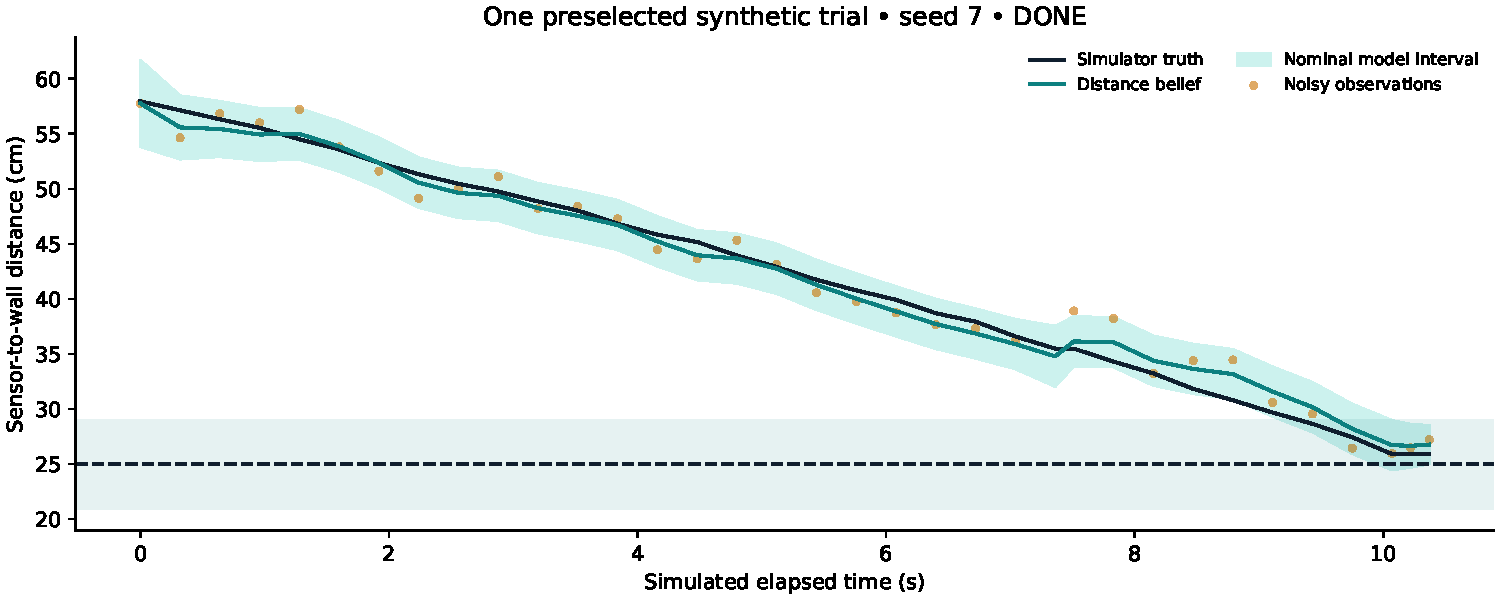
\includegraphics[width=\linewidth]{assets/belief_trace.pdf}
\par\small One preselected synthetic trace, seed 7. The shaded plot uses $1.96\sqrt P$ for display; the normal controller uses $1.64\sqrt P$ in its decisions. The plotted interval is not empirically calibrated coverage.\normalsize
\tuto{19}{Run the complete project on your laptop; chapter 20 interprets results}

\section{Physical experiment design and acceptance evidence}
Run stationary checks first, then supported wheels, then short floor pulses, then autonomous trials. Keep the broad cardboard wall, start range, floor and sensor reference consistent. Rotate policy order to avoid confounding policy with declining battery voltage. Record every attempt, including upload/runtime failures, aborts and user stops; do not silently remove inconvenient trials.

Measure final sensor-face distance independently with a ruler. Record policy, context, start/final distance, terminal event, time and any wall contact in \code{data/physical_trials_template.csv}. An operator stop is not a verified success; record it explicitly in notes and define its treatment before comparing results.

At least a small repeated pilot is needed to find mechanical problems; it does not establish high reliability. For an empirical success proportion $\hat p=s/N$, an approximate sampling standard error is $\sqrt{\hat p(1-\hat p)/N}$ under independent trials, but this estimate is misleading at zero/all successes. For example, with zero failures in $N$ independent representative trials, the exact one-sided 95\% upper failure probability solves $(1-p)^N=0.05$, giving $p=1-0.05^{1/N}$. This limits what a perfect small pilot can establish. Correlated trials and untested floors weaken even that interpretation.

Evaluate distance errors and failure types, not only completion rate. A model can be computationally correct but physically wrong because of biased sensing, wheel slip, timing or unsuitable geometry. Recalibrate after changing PWM, pulse duration, floor, batteries or sensor mounting.

\textbf{No physical validation has been performed for this package.} The 18 existing software tests and added mathematical checks verify stated computations and selected behaviours, not real-world safety or micro:bit resource compatibility.
\tuto{16}{Run your first floor trial; chapters 17--18 compare and record experiments}

\section{Reading route, source files and tutorial crosswalk}
\begin{longtable}{p{.35\linewidth}p{.22\linewidth}p{.31\linewidth}}
\toprule Mathematical question & This companion & Tutorial chapter (PDF page)\\\midrule\endhead
What is success? & Sections 1--2 & 01 (page 2)\\
What does the sensor measure? & Section 3 & 09 (page 10)\\
How does a pulse move the robot? & Sections 4, 12 & 07, 10 (pages 8, 11)\\
How is uncertainty updated? & Section 5 & 13 (page 14)\\
When should it stop or sample? & Sections 6--8 & 14 (page 15)\\
How does context matter? & Section 9 & 15 (page 16)\\
How do I check the arithmetic? & Section 10 & 13, 19 (pages 14, 20)\\
Where do the numbers come from? & Sections 11, 13 & 11--12 (pages 12--13)\\
How do I evaluate the result? & Sections 14--15 & 17--20 (pages 18--21)\\
\bottomrule
\end{longtable}
\textbf{Practical links:} \href{Tutorial_A_to_Z.pdf}{PDF tutorial}; \href{Tutorial_A_to_Z.html}{browser tutorial}; \href{index.html}{offline replay}; \href{README.md}{project README}.

\textbf{Implementation authority:} the files in \code{firmware/}: \code{belief_controller.py}, \code{hardware.py}, \code{main.py} and \code{config.py}. The seven generated \code{flash/} files embed these sources. Synthetic results come from \code{simulate.py}; calibration summaries from \code{tools/calibrate.py}. This document describes the current implementation rather than adding a different controller.

\textbf{Rebuild/check:} from the project directory, run the following commands. Run the second command twice to resolve the PDF cross-references.
{\small
\begin{verbatim}
python tools/check_math_model.py
pdflatex -interaction=nonstopmode -halt-on-error Mathematical_Model.tex
\end{verbatim}
}
The project archive includes editable LaTeX, numeric check output, the tutorial and its assets.

\begin{thebibliography}{9}
\bibitem{kalman} R. E. Kalman (1960). A New Approach to Linear Filtering and Prediction Problems. \emph{Journal of Basic Engineering} 82(1), 35--45. \href{https://doi.org/10.1115/1.3662552}{doi:10.1115/1.3662552}. Background for the scalar Gaussian recursion; project-specific guards and policy are derived above.
\bibitem{microbit} BBC micro:bit MicroPython V2 documentation. \emph{Machine: time\_pulse\_us}. \url{https://microbit-micropython.readthedocs.io/en/v2-docs/machine.html}. Accessed 10 September 2026.
\bibitem{kitronik} Kitronik. \emph{:MOVE Motor 5683}. \url{https://kitronik.co.uk/products/5683-kitronik-move-motor-for-the-bbc-micro-bit}. Driver source and retained licence are included in the project; see \code{docs/vendor_manifest.json} for pinned hashes. Physical calibration remains required.
\bibitem{picogk} LEAP 71. \emph{PicoGK: geometry kernel for computational engineering}. \url{https://picogk.org/}. Accessed 10 September 2026. The suggested bracket/enclosure use is our proposed extension.
\end{thebibliography}
\end{document}
